\documentclass[aspectratio=169]{beamer}

% Theme Choice
\usetheme{Madrid}
\usecolortheme{beaver}

% Packages
\usepackage{graphicx}
\usepackage{amsmath}
\usepackage{booktabs}
\usepackage{tikz}
\usetikzlibrary{calc, intersections}

% Title Information
\title{Unit 7: Resource Markets with Applications to Labor}
\subtitle{Factor Markets, Derived Demand, and Monopsony}
\author{Doğukan Günkördü}
\date{}

\begin{document}

% Slide 1: Title
\begin{frame}
    \titlepage
\end{frame}

% Slide 2: Learning Objectives
\begin{frame}{Learning Objectives}
    Based on Chapter 10, in this unit you will learn:
    \begin{itemize}
        \item \textbf{Product Markets vs. Resource Markets:} Understanding the connections.
        \item \textbf{Marginal Revenue Product (MRP):} Calculation and application.
        \item \textbf{Derived Demand:} Why firms hire workers.
        \item \textbf{Market Structures:} Perfectly Competitive Labor Markets vs. Monopsony.
        \item \textbf{Least-Cost Rule:} Optimizing combinations of labor and capital.
    \end{itemize}
\end{frame}

% Slide 3: Introduction to Factor Markets
\begin{frame}{Introduction to Factor Markets}
    \begin{block}{The Circular Flow Reversal}
        In previous units (Product Markets), individuals bought goods and firms sold them. In \textbf{Factor Markets}, roles are reversed:
    \end{block}
    
    \vspace{0.5cm}
    
    \begin{columns}
        \column{0.5\textwidth}
        \textbf{DEMANDERS (Buyers):}
        \begin{itemize}
            \item \textbf{Firms} search for inputs (Land, Labor, Capital, Entrepreneurship).
            \item Firms hire workers to produce goods.
        \end{itemize}
        
        \column{0.5\textwidth}
        \textbf{SUPPLIERS (Sellers):}
        \begin{itemize}
            \item \textbf{Individuals} supply their labor.
            \item Households own the factors of production.
        \end{itemize}
    \end{columns}
    
    \vspace{0.5cm}
    \textit{Example: A hospital demands doctors; a doctor supplies labor.}
\end{frame}

% Slide 4: Key Concept 1 - Derived Demand
\begin{frame}{Derived Demand}
    \begin{alertblock}{Definition: Derived Demand}
        Demand for resources (factors of production) is \textbf{derived} from the demand for the goods they produce.
    \end{alertblock}

    \vspace{0.5cm}
    \textbf{The Logic:}
    \begin{itemize}
        \item Consumers do not demand "shoemakers"; they demand "shoes."
        \item Because there is a demand for shoes, firms have a demand for shoemakers.
        \item \textbf{implication:} If demand for the product falls, demand for the labor produces it falls.
    \end{itemize}
\end{frame}

% Slide 5: Marginal Revenue Product (MRP)
\begin{frame}{Marginal Revenue Product (MRP)}
    To determine the value of a worker, we calculate MRP.
    
    \begin{block}{Definition}
        \textbf{MRP} is the addition to a firm's total revenue when an additional input (worker) is employed.
    \end{block}

    \begin{equation*}
        MRP = \frac{\Delta \text{Total Revenue}}{\Delta \text{Resource Quantity}}
    \end{equation*}

    \textbf{Alternative Formula (Perfect Competition):}
    \begin{equation*}
        MRP = \text{Marginal Product (MP)} \times \text{Price (P)}
    \end{equation*}
    
    \small{\textit{Note: In PC, $P = MR$, so $MRP = MP \times MR$.}}
\end{frame}

% Slide 6: Marginal Factor Cost (MFC)
\begin{frame}{Marginal Factor Cost (MFC)}
    Also called Marginal Resource Cost (MRC).
    
    \begin{block}{Definition}
        \textbf{MFC} is the additional cost to the firm of hiring one additional input (machine or worker).
    \end{block}

    \begin{equation*}
        MFC = \frac{\Delta \text{Total Resource Cost}}{\Delta \text{Resource Quantity}}
    \end{equation*}

    \begin{itemize}
        \item In a \textbf{Perfectly Competitive Labor Market}, firms are wage takers.
        \item Therefore: $\mathbf{MFC = Wage}$.
    \end{itemize}
\end{frame}

% Slide 7: The Profit-Maximizing Rule
\begin{frame}{Profit-Maximizing Rule for Resources}
    Just like $MR=MC$ in product markets, factor markets have a golden rule.
    
    \begin{alertblock}{The Rule}
        A firm maximizes profit by hiring resources up to the point where:
        \Huge
        \[ MRP = MFC \]
        \normalsize
    \end{alertblock}
    
    \vspace{0.3cm}
    \textbf{Logic:}
    \begin{itemize}
        \item If $MRP > MFC$: The worker brings in more money than they cost. \textbf{HIRE!}
        \item If $MRP < MFC$: The worker costs more than the revenue they generate. \textbf{FIRE (or don't hire)!}
    \end{itemize}
\end{frame}

% Slide 8: Shifters of Resource Demand
\begin{frame}{The Three Shifters of Resource Demand}
    The Demand for Labor (MRP) can shift due to:
    
    \begin{enumerate}
        \item \textbf{Changes in Product Demand:}
        \begin{itemize}
            \item Price of the product increases $\rightarrow$ MRP increases $\rightarrow$ Demand for labor shifts RIGHT.
        \end{itemize}
        
        \item \textbf{Changes in Productivity:}
        \begin{itemize}
            \item Technological progress increases Marginal Product (MP).
            \item Since $MRP = MP \times P$, productivity gains shift Demand for labor RIGHT.
        \end{itemize}
        
        \item \textbf{Changes in Price of Other Resources:}
        \begin{itemize}
            \item \textit{Substitute Resources:} If robot prices fall, demand for labor may fall (substitution effect).
            \item \textit{Complementary Resources:} If lumber gets cheaper, more houses are built, demand for construction workers rises.
        \end{itemize}
    \end{enumerate}
\end{frame}

% Slide 9: Perfectly Competitive Labor Market (Graphs)
\begin{frame}{Perfectly Competitive Labor Market}
    \begin{columns}
        \column{0.5\textwidth}
        \centering
        \textbf{The Market} \\
        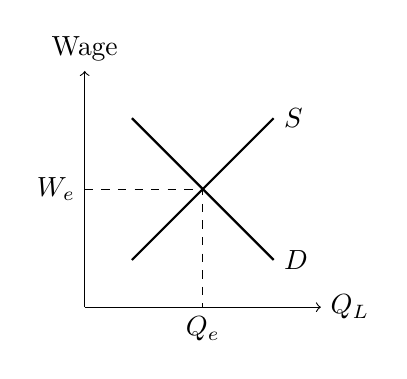
\begin{tikzpicture}[scale=0.6]
            \draw[->] (0,0) -- (5,0) node[right] {$Q_L$};
            \draw[->] (0,0) -- (0,5) node[above] {Wage};
            \draw[thick] (1,1) -- (4,4) node[right] {$S$};
            \draw[thick] (1,4) -- (4,1) node[right] {$D$};
            \draw[dashed] (0,2.5) node[left] {$W_e$} -- (2.5,2.5) -- (2.5,0) node[below] {$Q_e$};
        \end{tikzpicture}
        
        \column{0.5\textwidth}
        \centering
        \textbf{The Individual Firm} \\
        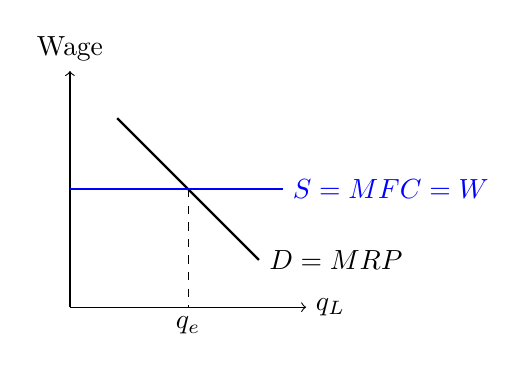
\begin{tikzpicture}[scale=0.6]
            \draw[->] (0,0) -- (5,0) node[right] {$q_L$};
            \draw[->] (0,0) -- (0,5) node[above] {Wage};
            \draw[thick] (1,4) -- (4,1) node[right] {$D=MRP$};
            \draw[thick, blue] (0,2.5) -- (4.5,2.5) node[right] {$S=MFC=W$};
            \draw[dashed] (2.5,2.5) -- (2.5,0) node[below] {$q_e$};
        \end{tikzpicture}
    \end{columns}
    
    \vspace{0.5cm}
    \begin{itemize}
        \item \textbf{Market:} Supply and Demand set the equilibrium wage ($W_e$).
        \item \textbf{Firm:} A "Wage Taker." Supply of labor is perfectly elastic (horizontal) at the market wage.
    \end{itemize}
\end{frame}

% Slide 10: Minimum Wage Impact
\begin{frame}{Minimum Wage (Price Floor)}
    What happens if the government sets an effective minimum wage above equilibrium?
    
    \vspace{0.3cm}
    \begin{itemize}
        \item \textbf{Wage Rate:} Increases ($W_{min} > W_e$).
        \item \textbf{Quantity Supplied ($Q_s$):} Increases (more people want to work).
        \item \textbf{Quantity Demanded ($Q_d$):} Decreases (firms hire fewer workers).
        \item \textbf{Result:} A surplus of labor (Unemployment).
    \end{itemize}
    
    \textit{Note: The individual firm faces a higher horizontal supply curve, so they move up along their MRP curve, hiring fewer workers.}
\end{frame}

% Slide 11: Monopsony
\begin{frame}{Monopsony}
    \begin{block}{Definition}
        A market where there is a \textbf{single buyer} of labor (e.g., a "company town" or coal mine).
    \end{block}

    \textbf{Characteristics:}
    \begin{itemize}
        \item "Monopoly of the factor market."
        \item The firm must increase wages to hire more workers.
        \item Because they must raise wages for \textit{all} workers to attract the next one, the Marginal Factor Cost (MFC) is \textbf{higher} than the Supply (Wage) curve.
    \end{itemize}
\end{frame}

% Slide 12: Monopsony Graph
\begin{frame}{Monopsony Graph Analysis}
    \begin{columns}
        \column{0.4\textwidth}
        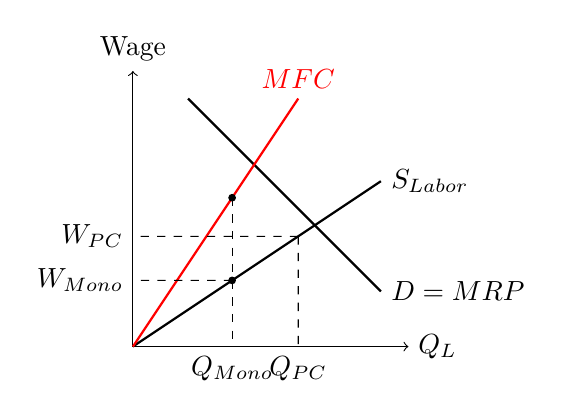
\begin{tikzpicture}[scale=0.7]
            \draw[->] (0,0) -- (5,0) node[right] {$Q_L$};
            \draw[->] (0,0) -- (0,5) node[above] {Wage};
            % MRP
            \draw[thick] (1,4.5) -- (4.5,1) node[right] {$D=MRP$};
            % Supply
            \draw[thick] (0,0) -- (4.5,3) node[right] {$S_{Labor}$};
            % MFC
            \draw[thick, red] (0,0) -- (3,4.5) node[above] {$MFC$};
            
            % Intersection MRP = MFC
            \coordinate (A) at (1.8, 2.7); % Approx intersection
            \fill (A) circle (2pt);
            
            % Quantity Line
            \draw[dashed] (1.8, 2.7) -- (1.8,0) node[below] {$Q_{Mono}$};
            
            % Wage Line (Down to Supply)
            \coordinate (B) at (1.8, 1.2); % Point on Supply curve
            \fill (B) circle (2pt);
            \draw[dashed] (B) -- (0,1.2) node[left] {$W_{Mono}$};
            
            % Comparison to Competitive
            \coordinate (C) at (3,2); % Supply = Demand
            \draw[dashed] (C) -- (3,0) node[below] {$Q_{PC}$};
             \draw[dashed] (C) -- (0,2) node[left] {$W_{PC}$};
        \end{tikzpicture}
        
        \column{0.6\textwidth}
        \textbf{Steps to find Equilibrium:}
        \begin{enumerate}
            \item Find Quantity where $MRP = MFC$ (Profit Max).
            \item Go \textbf{down} to the Supply Curve to find the Wage ($W_{Mono}$).
        \end{enumerate}
        
        \vspace{0.3cm}
        \textbf{Comparison to Perfect Competition:}
        \begin{itemize}
            \item Monopsonies hire \textbf{fewer} workers ($Q_{Mono} < Q_{PC}$).
            \item Monopsonies pay a \textbf{lower} wage ($W_{Mono} < W_{PC}$).
        \end{itemize}
    \end{columns}
\end{frame}

% Slide 13: Least-Cost Rule
\begin{frame}{Least-Cost Rule}
    Firms use multiple inputs (Labor and Capital). To minimize costs for a specific output level, they follow the \textbf{Least-Cost Rule}.
    
    \begin{block}{Formula}
        \[ \frac{MP_L}{P_L} = \frac{MP_K}{P_K} \]
        \small{Where $L$ is Labor and $K$ is Capital.}
    \end{block}
    
    \textbf{Optimization Logic:}
    \begin{itemize}
        \item If $\frac{MP_L}{P_L} > \frac{MP_K}{P_K}$: Labor gives more "bang for the buck." \textbf{Buy more Labor, less Capital.}
        \item As you hire more Labor, $MP_L$ falls (Diminishing Returns), eventually equalizing the ratios.
    \end{itemize}
\end{frame}

% Slide 14: Practical Example (Table 10.2 Logic)
\begin{frame}{Least-Cost Example}
    \textbf{Scenario:}
    \begin{itemize}
        \item Price of Labor ($P_L$) = \$5
        \item Price of Robots ($P_K$) = \$10
        \item Budget = \$35
    \end{itemize}

    \textbf{Decision Process:}
    \begin{enumerate}
        \item Calculate Marginal Product per Dollar ($MP/P$) for both.
        \item Select the resource with the highest $MP/P$.
        \item Repeat until budget is spent.
    \end{enumerate}
    
    \vspace{0.2cm}
    \textit{Result:} The firm adjusts inputs until the last dollar spent on labor yields the same marginal product as the last dollar spent on robots.
\end{frame}

% Slide 15: Summary
\begin{frame}{Unit Summary}
    \begin{itemize}
        \item \textbf{MRP = MFC:} The golden rule for hiring quantity.
        \item \textbf{Perfect Competition:} Firm is a wage taker ($Supply = MFC = Wage$).
        \item \textbf{Monopsony:} Single buyer, MFC > Supply. They under-hire and under-pay compared to competitive markets.
        \item \textbf{Least-Cost Rule:} $\frac{MP_L}{P_L} = \frac{MP_K}{P_K}$.
        \item \textbf{Shifters:} Remember that demand for labor is \textbf{Derived Demand}.
    \end{itemize}
\end{frame}

\end{document}
